
\noindent \textbf{L2.1 (Sipser 1.16)} Resolva o exercício 1.16.\\[3pt]
\noindent\textbf{a) Resposta:} Seja $N$ o AFN dado na questão e $A$ a linguagem reconhecida por $N$, onde:\\[6pt]
\noindent$N = \{Q, \Sigma, \delta, q_{0}, F\}$\\
$Q = \{1,2\}$\\
$\Sigma = \{a, b\}$\\
$q_0 = 1$\\
$F = \{1\}$\\
$\delta = $
\begin{table}[!h]
\centering
\rot{\hspace{5 mm}\llap{Estados}}
\begin{tabular}{l|l|l}
        & a          & b        \\ \hline
1       & \{1, 2\}   & \{2\}    \\
2       & \{\}       & \{1\}    \\
\end{tabular}
\end{table}

Agora, vamos construir um AFD $M = \{Q', \Sigma, \delta', q_{0'}, F'\}$, equivalente à $N$, que reconhece $A$.

\noindent$Q' = \{\{\}, \{1\}, \{2\}, \{1,2\} \}$\\
$\Sigma = \{a, b\}$\\
$q_{0'} = E(\{1\}) = \{1\}$\\
$F' = \{\{1\}, \{1,2\}\}$\\
$\delta' = $
\begin{table}[!h]
\centering
\rot{\hspace{5 mm}\llap{Estados}}
\begin{tabular}{l|l|l}
         & a         & b        \\ \hline
\{\}     & \{\}      & \{\}     \\
\{1\}    & \{1,2\}   & \{2\}    \\
\{2\}    & \{\}      & \{1\}    \\
\{1,2\}  & \{1,2\}   & \{1,2\}
\end{tabular}
\end{table}

\begin{figure}[H]
\centering
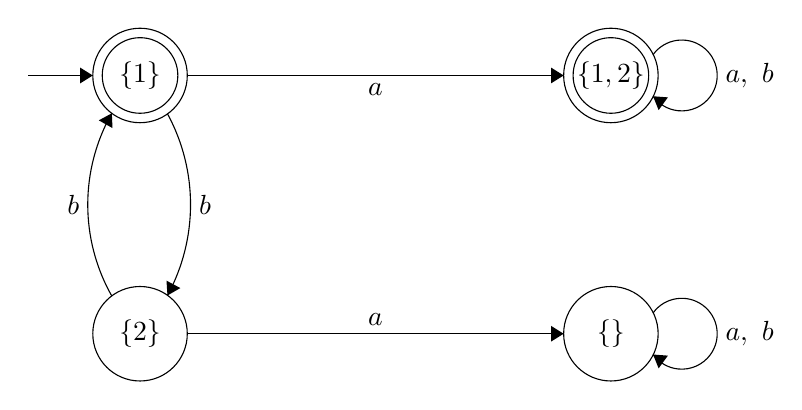
\begin{tikzpicture}[scale=0.2]
\tikzstyle{every node}+=[inner sep=0pt]
\draw [black] (17.6,-19.6) circle (3);
\draw (17.6,-19.6) node {$\{1\}$};
\draw [black] (17.6,-19.6) circle (2.4);
\draw [black] (47.5,-36) circle (3);
\draw (47.5,-36) node {$\{\}$};
\draw [black] (17.6,-36) circle (3);
\draw (17.6,-36) node {$\{2\}$};
\draw [black] (47.5,-19.6) circle (3);
\draw (47.5,-19.6) node {$\{1,2\}$};
\draw [black] (47.5,-19.6) circle (2.4);
\draw [black] (19.342,-22.033) arc (28.49627:-28.49627:12.088);
\fill [black] (19.34,-33.57) -- (20.16,-33.1) -- (19.28,-32.63);
\draw (21.31,-27.8) node [right] {$b$};
\draw [black] (50.18,-34.677) arc (144:-144:2.25);
\draw (54.75,-36) node [right] {$a,\mbox{ }b$};
\fill [black] (50.18,-37.32) -- (50.53,-38.2) -- (51.12,-37.39);
\draw [black] (20.6,-36) -- (44.5,-36);
\fill [black] (44.5,-36) -- (43.7,-35.5) -- (43.7,-36.5);
\draw (32.55,-35.5) node [above] {$a$};
\draw [black] (15.808,-33.604) arc (-150.49236:-209.50764:11.784);
\fill [black] (15.81,-22) -- (14.98,-22.45) -- (15.85,-22.94);
\draw (13.78,-27.8) node [left] {$b$};
\draw [black] (50.18,-18.277) arc (144:-144:2.25);
\draw (54.75,-19.6) node [right] {$a,\mbox{ }b$};
\fill [black] (50.18,-20.92) -- (50.53,-21.8) -- (51.12,-20.99);
\draw [black] (20.6,-19.6) -- (44.5,-19.6);
\fill [black] (44.5,-19.6) -- (43.7,-19.1) -- (43.7,-20.1);
\draw (32.55,-20.1) node [below] {$a$};
\draw [black] (10.5,-19.6) -- (14.6,-19.6);
\fill [black] (14.6,-19.6) -- (13.8,-19.1) -- (13.8,-20.1);
\end{tikzpicture}
\caption{Diagrama de estados para o AFD $M$.}
\label{fig:sip1.16a}
\end{figure}

% item b) %
\noindent\textbf{b) Resposta:} Seja $N$ o AFN dado na questão e $A$ a linguagem reconhecida por $N$, onde:\\[6pt]
\noindent$N = \{Q, \Sigma, \delta, q_{0}, F\}$\\
$Q = \{1, 2, 3\}$\\
$\Sigma = \{a, b\}$\\
$q_0 = 1$\\
$F = \{2\}$\\
$\delta = $
\begin{table}[!h]
\centering
\rot{\hspace{5 mm}\llap{Estados}}
\begin{tabular}{l|l|l|l}
     & a        & b         & $\epsilon$ \\ \hline
1    & \{3\}    & \{\}      & \{2\}    \\
2    & \{1\}    & \{\}      & \{\}    \\
3    & \{2\}    & \{2, 3\}  & \{\}    \\
\end{tabular}
\end{table}

Agora, vamos construir um AFD $M = \{Q', \Sigma, \delta', q_{0'}, F'\}$, equivalente à $N$, que reconhece $A$.

\noindent$Q' = \{\{\}, \{1\}, \{2\}, \{3\}, \{1,2\}, \{1,3\}, \{2,3\}, \{1,2,3\} \}$\\
$\Sigma = \{a, b\}$\\
$q_{0'} = E(\{1\}) = \{1,2\}$\\
$F' = \{\{2\}, \{1,2\}, \{2,3\}, \{1,2,3\} \}$\\
$\delta' = $
\begin{table}[!h]
\centering
\rot{\hspace{5 mm}\llap{Estados}}
\begin{tabular}{l|l|l}
            & a             & b         \\ \hline
\{\}        & \{\}          & \{\}      \\
\{1\}       & \{3\}         & \{\}      \\
\{2\}       & \{1,2\}       & \{\}      \\
\{3\}       & \{2\}         & \{2,3\}   \\
\{1,2\}     & \{1,2,3\}     & \{\}      \\
\{1,3\}     & \{2,3\}       & \{2,3\}   \\
\{2,3\}     & \{1,2\}       & \{2,3\}   \\
\{1,2,3\}   & \{1,2,3\}     & \{2,3\}
\end{tabular}
\end{table}

\begin{figure}[!ht]
\centering
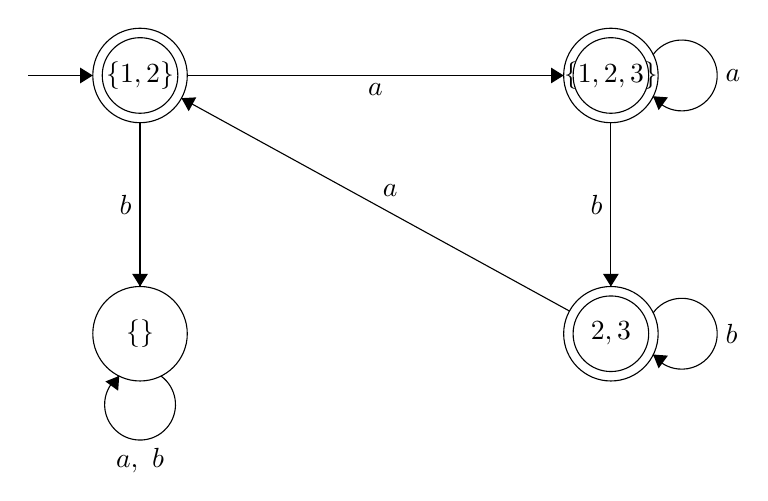
\begin{tikzpicture}[scale=0.2]
\tikzstyle{every node}+=[inner sep=0pt]
\draw [black] (17.6,-19.6) circle (3);
\draw (17.6,-19.6) node {$\{1,2\}$};
\draw [black] (17.6,-19.6) circle (2.4);
\draw [black] (47.5,-36) circle (3);
\draw (47.5,-36) node {${2,3}$};
\draw [black] (47.5,-36) circle (2.4);
\draw [black] (17.6,-36) circle (3);
\draw (17.6,-36) node {$\{\}$};
\draw [black] (47.5,-19.6) circle (3);
\draw (47.5,-19.6) node {$\{1,2,3\}$};
\draw [black] (47.5,-19.6) circle (2.4);
\draw [black] (50.18,-34.677) arc (144:-144:2.25);
\draw (54.75,-36) node [right] {$b$};
\fill [black] (50.18,-37.32) -- (50.53,-38.2) -- (51.12,-37.39);
\draw [black] (50.18,-18.277) arc (144:-144:2.25);
\draw (54.75,-19.6) node [right] {$a$};
\fill [black] (50.18,-20.92) -- (50.53,-21.8) -- (51.12,-20.99);
\draw [black] (20.6,-19.6) -- (44.5,-19.6);
\fill [black] (44.5,-19.6) -- (43.7,-19.1) -- (43.7,-20.1);
\draw (32.55,-20.1) node [below] {$a$};
\draw [black] (10.5,-19.6) -- (14.6,-19.6);
\fill [black] (14.6,-19.6) -- (13.8,-19.1) -- (13.8,-20.1);
\draw [black] (17.6,-22.6) -- (17.6,-33);
\fill [black] (17.6,-33) -- (18.1,-32.2) -- (17.1,-32.2);
\draw (17.1,-27.8) node [left] {$b$};
\draw [black] (18.923,-38.68) arc (54:-234:2.25);
\draw (17.6,-43.25) node [below] {$a,\mbox{ }b$};
\fill [black] (16.28,-38.68) -- (15.4,-39.03) -- (16.21,-39.62);
\draw [black] (47.5,-22.6) -- (47.5,-33);
\fill [black] (47.5,-33) -- (48,-32.2) -- (47,-32.2);
\draw (47,-27.8) node [left] {$b$};
\draw [black] (44.87,-34.56) -- (20.23,-21.04);
\fill [black] (20.23,-21.04) -- (20.69,-21.87) -- (21.17,-20.99);
\draw (33.49,-27.3) node [above] {$a$};
\end{tikzpicture}
\caption{Diagrama de estados para o AFD $M$.}
\label{fig:sip1.16b}
\end{figure}

A figura \ref{fig:sip1.16b} é o AFD simplificado que mostra apenas os estados que são alcançáveis a partir do estado inicial $\{1,2\}$.\\[6pt]